%%%%%%%%%%%%%%%%%%%%%%%%%%%%%%%%%%%%%%%%%%%%%%%%%%%%%%%%%%%%%%%%%%
%%%%%%%% ICML 2010 EXAMPLE LATEX SUBMISSION FILE %%%%%%%%%%%%%%%%%
%%%%%%%%%%%%%%%%%%%%%%%%%%%%%%%%%%%%%%%%%%%%%%%%%%%%%%%%%%%%%%%%%%

% Use the following line _only_ if you're still using LaTeX 2.09.
%\documentstyle[icml2010,epsf,natbib]{article}
% If you rely on Latex2e packages, like most moden people use this:
\documentclass{article}

% For figures
\usepackage{graphicx} % more modern
%\usepackage{epsfig} % less modern
\usepackage{subfigure} 

% For citations
\usepackage{natbib}

% For algorithms
\usepackage{algorithm}
\usepackage{algorithmic}

% As of 2010, we use the hyperref package to produce hyperlinks in the
% resulting PDF.  If this breaks your system, please commend out the
% following usepackage line and replace \usepackage{icml2010} with
% \usepackage[nohyperref]{icml2010} above.
\usepackage{hyperref}

% Packages hyperref and algorithmic misbehave sometimes.  We can fix
% this with the following command.
\newcommand{\theHalgorithm}{\arabic{algorithm}}

% Employ the following version of the ``usepackage'' statement for
% submitting the draft version of the paper for review.  This will set
% the note in the first column to ``Under review.  Do not distribute.''
\usepackage{icml2010} 

% Employ this version of the ``usepackage'' statement after the paper has
% been accepted, when creating the final version.  This will set the
% note in the first column to ``Appearing in''
% \usepackage[accepted]{icml2010}

\newcommand{\F}{\mathcal{F}}
\newcommand{\PY}{\mathcal{P}\mathcal{Y}}
\newcommand{\G}{\mathcal{G}}
\newcommand{\ES}{\mathcal{E}\mathcal{S}}
\newcommand{\DP}{\mathcal{D}\mathcal{P}}

% The \icmltitle you define below is probably too long as a header.
% Therefore, a short form for the running title is supplied here:
\icmltitlerunning{Forgetting Counts}

\begin{document} 

\twocolumn[
\icmltitle{Constant Memory Inference \\
of Discrete Dependent Hierarchical Pitman-Yor Processes}

% It is OKAY to include author information, even for blind
% submissions: the style file will automatically remove it for you
% unless you've provided the [accepted] option to the icml2010
% package.
\icmlauthor{Nicholas Bartlett}{bartlett@stat.columbia.edu}
\icmladdress{Columbia University,
Room 1005 SSW, MC 4690,
1255 Amsterdam Avenue, New York, NY 10027}

\icmlauthor{Frank Wood}{fwood@stat.columbia.edu}
\icmladdress{Columbia University,
Room 1005 SSW, MC 4690,
1255 Amsterdam Avenue, New York, NY 10027}

% You may provide any keywords that you 
% find helpful for describing your paper; these are used to populate 
% the "keywords" metadata in the PDF but will not be shown in the document
\icmlkeywords{compression Pitman-Yor memory}

\vskip 0.3in
]

\begin{abstract} 
We propose a hierarchical Bayesian nonparametric model for discrete sequence data that can be represented in constant space and estimated incrementally in linear time.  The resulting estimation procedure can be viewed as either approximate inference
\end{abstract} 

\section{Introduction}

Nonparametric models, Bayesian or not, are characterized by computational and memory complexities that grow as a function of the size of the training data.  Unfortunately in common practice the relationship between training dataset size and complexity is used to select a dataset whose size is sufficiently small to allow model estimation.  Clearly this is not ideal given a sufficiently large and complex dataset.

When the computer is fixed but the dataset is not of fixed size but instead grows monotonically, two constraints are imposed on the computational complexity of inference and estimation procedures.  First, the computational complexity of estimation and inference cannot be greater than linear in the size of the data.  Second, the memory complexity of such algorithms must be constant.  Also, particularly in the case of growing data, the only suitable estimation and inference procedures are those that are incremental in nature.

In this paper we develop a {\em constant space, linear time} incremental estimation procedure for models of discrete sequence data based on the hierarchical Pitman-Yor process (HPYP) \cite{Teh2006a}.   Our contribution can be described as a ``forgetting'' procedure that retains only a constant-sized subset of the training dataset.  Inference in the resulting model can be interpreted as either proper inference in a sequence of dependent HPYP's or as approximate inference in a single non-varying HPYP.  To achieve this result we draw on recent results in HPYP estimation, namely the marginalization operations highlighted in the sequence memoizer \cite{Wood2009} and results from dependent Dirichlet process estimation, namely the generalized Polya urn scheme \cite{Caron2007}.  

Our motivation for this work is the sequence memoizer (SM) \cite{Wood2009} which was demonstrated to be a good predictive model for discrete sequence data.  An  {\em linear space, linear time} incremental estimator for the SM was developed and used in a file compression setting \cite{Gasthaus2010}.

If the memory complexity of the estimated model is constant with respect to training data size then both no more than a constant number of datapoints can be retained and no more than a constant number of parameters can be used.  It seems strange then to consider constant memory inference for a nonparametric model because, fundamentally, the resulting constant memory model estimate must be parametric.

Regardless, the Gaussian process regression literature, for one example, includes many such approaches anyway \cite{gaussian process regression stuff, lawrence, csato, snelson, etc}.  The reason for this is that estimation of Gaussian process regression models requires $O(n^2)$ space and $O(n^3)$ time where $n$ is the (growing) number of observations,  hindering their widespread use.  

%Inference in a simple (non-sparse) nonparametric kernel density estimator (assuming the kernel has broad support) requires access to all of the training data.  Large, fixed size datasets can often be accommodated by either engineering strategies (parallelism, etc.)~or approximation schemes (careful selection of representative subsets of the data).  Of course, fixed size data 

\comment{
%Bayesian nonparametric models interpolate between nonparametric 

%It can be difficult to distinguish between ``number of parameters,'' model ``complexity,'' and 


Parametric and nonparametric models differ in several key ways.  One important way is that parametric models have a fixed, finite number of parameters whereas nonparametric models are often described as having an effective number of ``parameters'' (often the datapoints or a subset of the datapoints themselves) that grows as a function of the size of the training data.

%An example of the former is Gaussian mixture model.  An example of the latter is a kernel density estimator.  In the former the number of mixture components is fixed a priori and the inference goal might be, in the case of density estimation, to find parameters that maximize the probability of the training data under the model.  In the latter, kernel density estimation case, the ``parameters'' of the model are the data points themselves (and perhaps parameters for a kernel function).  Here the effective number of parameters clearly grows linearly in the size of the training data. 

Bayesian nonparametric (BNP)  models are, somewhat confusingly, described as having ``complexity'' that grows as a function of the number of training data observations \cite{griffiths}.  BNP models are characterized by infinite dimensional parameter spaces \cite{sethurman, gaussian process function space reference}.   The former perspective derives from the fact that many BNP models can be ``collapsed'' in the sense that the infinite dimensional parameter space can be marginalized out yielding a simple, finite (for any finite dataset) representation whose memory complexity grows as a function of the training data size  (Chinese restaurant process \cite{CRP}, Polya urn representation \cite{poly urn}, etc.).  



%As a concrete example consider sequential importance sampling inference for a exponential family (conjugate) Dirichlet process mixture \cite{DP particle filter work}.  a fully collapsed representation can be used in which only the counts per class and sufficient statistics for each class need to be represented.


In such schemes, instead of representing the full infinite dimensional parameter space (or a truncation of it \cite{blei variational stuff}), such a collapsed representation instead only realizes and represents that part of the infinite dimensional parameter space ``responsible'' for generating the training data.     

%This difference in description is perhaps best explained through an example.  In a model with a Dirichlet process prior like $x_i | \G \sim \G, \G|\alpha,\G_0 \sim \DP(\alpha, \G_0),\; i=1\ldots n$,  either the posterior distribution of $\G |  \{x_i\}_{i=1}^{n},\alpha,\G_0$ or the posterior predictive distribution of $x_{n+1} | \{x_i\}_{i=1}^{n},\alpha,\G_0$ may be of interest.   In the former case, since it is known that both a priori and a posteriori that $\G$ has the form $\G = \sum_{k=1}^\infty \pi_k \delta_{\phi_k}$ \cite{sethurman} it is clear that the number of parameters in the model is infinite (there are an infinite number of so-called ``sticks,'' $\pi_k$ and ``atoms'' $\phi_k$).  On the other hand, ``marginal'' posterior predictive inference can be performed in such a model with $\G$ analytically integrated out.  Such inference utilizes representations in which the ``effective'' number of parameters in the model (really the state required to represent a single exact sample) grows in expectation as a function of the number of training data observations (Polya urn and Chinese restaurant process samplers \cite{plya_urn, crp} for example).  Other BNP models exhibit similar characteristics.

There is a connection between the effective number of parameters and the storage requirement for 

While nonparametric approaches (\cite{lots of shit}) in general, and BNP approaches in particular (\cite{lots more shit}) have exhibited empirical promise in a wide variety of application domains, enthusiasm for such methods should be damped by the realization that even sub-linear growth in the effective number of parameters is extremely problematic.  This is because, for any ``life-long'' learning agent, or any inference procedure exposed to extremely large training data sets, such growth will eventually make inference prohibitively expensive.  

In the BNP literature, this issue most acutely arises in Gaussian process (GP) models, where storage and computational complexity grow quadratically and cubically in the training data size.  To apply GP models to datasets of more than a few thousand data points requires using sparse variants that all effectively choose a ``best'' subset of the training data instances \cite{snelson, csato, etc}.  



How much memory must be used to represent such a model is highly dependent on the inference approach (approximate versus exact) and the representation used (one parameter per observation, one parameter per table and assignment to tables)

%(a Gaussian process is parameterized by mean and covariance {\em functions}, a Dirichlet process by a  

%``speak for themselves''


%The task of general file compression with an algorithm requiring constant space is of obvious practical value.  In any application there will be only a finite amount of memory available and many excellent compression algorithms become unfeasible when compressing large files.  In order to address this task directly an algorithm which allows a specified maximum memory allocation prior to running is needed.  In the case of compression through the use of probabilistic models, the algorithm should control the amount of memory required by adapting the complexity of the model in an appropriate manner to accommodate the stated memory bounds.

%Probabilistic models have been shown to perform extremely well when combined with an entropy encoder in compression algorithms.  These models work by predicting the next type in a sequence of types, most often bytes, which make up a file.  The better the model is, the more efficient the encoding scheme and the higher the compression ratio.  The model referred to as a stochastic memoizer for sequence data [wood] has recently been shown to outperform several other such models for general compression tasks [Gasthaus].  Unfortunately many of these byte level prediction algorithms require space on the order of the sequence length and thus become unrealistic for very large files.

%Even for models with theoretically constant memory requirements, such as n-gram models, the memory restriction cannot be pre-specified and the theoretical value is such a gross overestimate of the likely memory requirements it does not provide insight regarding the parameterization of the model at the start.  In section 1 of this paper we will review the stochastic memoizer for sequence data [wood].
}


\section{The basic model}

\subsection{Pitman-Yor Process}

The Pitman-Yor process is a generalization of the Dirichlet process and is a distribution over distributions with three parameters.  If $\G_1 \sim \PY(d,c,\G_0)$ we say $\G_1$ is distributed according to a Pitman-Yor process with discount parameter $d$, concentration parameter $c$, and base measure $\G_0$. The Pitman-Yor process reduces to the Dirichlet process when $d = 0$ \cite{Pitman}. 

The Pitman-Yor process can also be reformulated by analytically marginalizing out the random distribution $\G_1$.  To draw a sample $\{ \theta_j \}_{j = 1}^N$ in this representation we use a two step process.  The first step is to obtain a partition of the first $N$ integers from the two parameter Ewen's sampling distribution ($\ES_N(d,c)$).  The second step is to endow each of the $K$ parts of the partition with a parameter $\psi_k$ drawn independently from $\G_0$.  We define $\theta_j = \psi_k$ for all integers $j$ in the $k$'th section of the partion \cite{mcqueen??}.

The two parameter Ewen's sampling distribution is most easily understood through the process by which a sample is generated.  The process is known as the Chinese restaurant process (CRP) because of the metaphor that integers correspond to customers being seating in a restaurant with infinitely many tables.  Since the details of this process are critical for extensions made later we need to describe the CRP in detail. The process is initialized by seating the first customer at an empty table.  Customers $2 \dots N$ are seated sequentially by seating the $j$'th customer at a table drawn from the following distribution:

\begin{eqnarray*}
p(\textrm{table}_i, i<= t_{j-1} |\textrm{ previous customers}) &=& \frac{n_i - d}{j-1+ c}\\
p(\textrm{table}_{t_{j-1} +1} | \textrm{ previous customers}) &=& \frac{t_{j-1}d +c}{j-1+c}
\end{eqnarray*}

where $n_i$ is the number of customers already sitting at table $i$ and $t_{j-1}$ is the number of tables occupied by the first $j-1$ customers.  The final state of the restaurant defines a partition over the first $N$ integers which follows the $\ES_N(d,c)$ distribution.  Step two of the algorithm above is achieved by endowing each table with a parameter $\psi_k$ drawn independently from $\G_0$.

%TODO need a figure here to show restaurants arranged.  rest 1 will be the upper restaurant, rest 2 will be the lower restaurant.
These random distributions can be arranged in a hierarchy, such as the case that $\G_2 \sim \PY(d_2, c_2, \G_1)$ and $\G_1 \sim \PY(d_1, c_1, \G_0)$.  The hierarchical process can also be reformulated by analytically marginalizing out both $\G_2$ and $\G_1$.  Samples are obtained by iterating the algorithm for the single Pitman-Yor process.  To draw a sample $\{ \theta_j \}_{j = 1}^N$ we again need to obtain a partition of the first $N$ integers from $\ES_N(d,c)$.  This can be achieved through the CRP.  We will call this restaurant the child restaurant and denote the number of tables as $K_2$.  Each of the $K_2$ tables must be endowed with a parameter $ \psi_{2k}$ drawn independently from $\G_1$.  Since $\G_1$ has been marginalized out we can obtain $\{ \psi_{2k} \}_ {k = 1}^{K_2}$ by again using the algorithm for the single Pitman-Yor process.  A partition from the $\ES_{K_2}(d,c)$ is generated via the CRP.  We will call this restaurant the parent restaurant and the number of tables $K_1$.   Each of the $K_1$ tables must be endowed with a parameter $\psi_{1k}, k = 1 \ldots K_1$,  independently drawn from $\G_0$.  The sample consists of $\theta_j =\psi_{2k}$ for all customers $j$ sitting at table $k$ in the the child restaurant.

The process is most easily understood by looking at Figure~\ref{figHPY} in which the CRP process for the child restaurant resulted in three tables ($K_2 = 3$).  Therefore, three parameters must be drawn from $\G_1$.  Since $\G_1$ is marginalized we again revert to the process for a single Pitman-Yor process. The CRP for the parent restaurant resulted in two tables ($K_1 = 2$).  $\psi_{11}$ and $\psi_{12}$ are drawn independently from the base distribution $\G_0$.  $\{ \psi_2k \}_{k = 1}^{K_1}$ is then equal to $\{ \theta_1, \theta_1, \theta_2 \}$ which are then the parameters endowed to tables in the child restaurant.  From the figure we find that  $\{ \theta_j \}_{j = 1}^7 = \{ \theta_1, \theta_1, \theta_2, \theta_1, \theta_1, \theta_1, \theta_1 \}$.

The iterative application of the CRP representation is known as the Chinese restaurant franchise (CRF) \cite{teh hdp paper}.  As alluded to in Figure~\ref{figHPY}, the number of child restaurants is not restricted to one.  Furthermore, the iterative nature of the process makes extensions to deeper hierarchies natural.  For more extensive coverage of these representations we refer the reader to \cite{teh hpp} and \cite{teh hpy for langmodel}.

\subsection{Sequence Memoizer}

The sequence memoizer (SM) \cite{wood}, is a hierarchical Pitman-Yor model of unbounded depth for discrete sequence data.  Each node in the graphical model represents the distribution over the set of types ($\Sigma$) conditioned by a unique context.  The context consists of the entire sequence of types preceding the observation.  We can write the model as:

\begin{eqnarray*}
	\G_{[]} | \mathcal{U}_{\Sigma}, d_0 &\sim& \PY(d_0, 0, \mathcal{U}_{\Sigma }) \\
	\G_{\bf{u}} | \G_{\sigma(\bf{u})}, d_{|\bf{u}|} &\sim& \PY(d_{|\bf{u}|}, 0, \G_{\sigma(\bf{u})}) \hspace{1cm} \forall \bf{u} \in \Sigma^+
\end{eqnarray*}

where $\mathcal{U}_{\Sigma }$ is a uniform distribution over the set of types, $\bf{u}$ is a particular context, $\Sigma^+$ is the set of all such contexts, and $\sigma(\bf{u})$ is the context $\bf{u}$ modified by removing the most distant type.  We assume $| \Sigma | < \infty$.

In \cite{pitman} they show that  if $\G_2 \sim \PY(d_2, 0, \G_1)$ and  $\G_1 \sim \PY(d_1, 0, \G_0)$ then marginally, $\G_2 \sim \PY(d_2 d_2, 0, \G_0)$.  \cite{wood} applied this result to show that the graphical model for the SM to be identified in linear time and initiated in linear space.

Inference in the SM model is performed in the Chinese restaurant franchise respresentation. Inference takes worst case $\mathcal{O}(n^2)$ time and requires $\mathcal{O}(n)$ space. Quadratic time stems from the fact that seating a customer in the appropriate restaurant may require seating a customer in all of the restaurants above it.  The length of this path is bounded by the length of the sequence. Each restaurant requires constant space because a restaurant need only maintain a constant number of summary statistics, the total number of customers and the total number of tables present of each type.\footnote{For symbol sets of finite cardinality.} Note this representation requires reinstantiation of the full restaurant state for some steps of inference which can be done by exploiting exchangeability.


\section{Theory}
\label{sec:theory}

While the SM model demonstrates promising empirical results \cite{Gasthaus} we are unsatisfied with the linear space requirement for reasons stated earlier.  We propose a framework for limiting the memory required to represent models based on the hierarchical Pitman-Yor process.  Estimation in this framework can be viewed either as a valid inference scheme for a model based on a dependent set of hierarchical Pitman-Yor processes or as an approximate inference technique for a non-varying model.

\subsection{Dependent Pitman-Yor process} 

The $\ES_N(d,c)$ distribution discussed in Section~\ref{basicModel} has an important consistency property. In the Chinese restaurant metaphor the consistency property corresponds to the fact that if a customer is removed uniformly at random, the remaining customer configuration represents a partition of the integer $N-1$ following the $\ES_{N-1}(d,c)$ distribution. Another deletion operation known as size-biased deletion, in which a customer is chosen uniformly at random and all customers seated at the same table are removed from the restaurant, is known to satisfy such a consistency property for the one parameter Ewen's distribution \cite{kingman}.  This is known as the species deletion property \cite{kingman}, but does not hold in the two parameter case \cite{pitman}

The consistency property allows the restaurant representation to be modified to draw samples  $\{ \theta_j^t \}_{i = 1}^{N_t}$ from a sequence of dependent random distributions $\{ \G^t \}_{t=1}^T$ such that 
%
\begin{eqnarray}
 \label{eqnDependentPY1}  \G^t | d, c, \G_0 &\sim& \PY(d,c,\G_0)\\
 \label{eqnDependentPY2}  \theta_j^t | \G^t &\sim& \G^t \hspace{.5cm} j = 1 \dots N_t.
 \end{eqnarray}
 %
We use the index $t$ because of the useful interpretation as time even though it need not be a temporal sequence. The fact that $\G^t_1$ has the same distribution over time is known as stationarity \cite{davis and brockwel}.  
 
The generative procedure, an extension of the analogous procedure for dependent Dirichlet processes \cite{caron}, starts with an empty restaurant and generates $\{ \theta_j^1\}_{i = 1}^{N_1}$ by using the CRP to generate a partition of the integer $N_1$ and then endowing each table with a value drawn independently from $\G_0$.  Between time points customers are deleted uniformly at random from the customer configuration of the restaurant and empty tables are removed from the restaurant.  After the deletion step new customers are seated according to the CRP with the initial customer configuration of the process given by the configuration resulting from the deletion step.  Once new customers have been seated, previously unoccupied tables are endowed with a value drawn independently from $\G_0$.  We set $\theta^t_j = \psi_k$ if  the $j^{th}$ customer seated during the $t^{th}$ time step is seated at table $k$.

If $j$ customers are deleted after time step 1 the partition represented by the starting customer configuration of the restaurant at time step 2 follows a $\ES_{N_1- j}(d,c)$ distribution.  Therefore, after seating new customers in time step 2 the configuration results in partition which follows a $\ES_{N_1 - j + N_2}(d,c)$ distribution.  This is the only result needed to ensure Eqn.~\ref{eqnDependentPY1} and Eqn.~\ref{eqnDependentPY2}.  Note that the number of customers removed from the restaurant between time steps is independent of the consistency result and can thus be either stochastic or deterministic.

Dependence between $\G^t$ is induced by the modified restaurant representation through the undeleted customers.  An exact characterization of the dependence is non-trivial.   \cite{caron} show that in the analogous procedure for dependent Dirichlet distributions, removing fewer customers between time steps induces higher dependence.  In the extreme case of removing all the customers between time steps, the procedure generates samples drawn from independent $\G^t$. Removing no customers implies a $\G$ that is not varying with the index $t$. 

%TODO give graphical model
\subsection{Time-varying Pitman-Yor Process in a hierarchical setting}

Consider now the hierarchical dependent setting 
%
\begin{eqnarray*}
\G_1 | d_1, c_1, \G_0 &\sim& \PY(d_1, c_1, \G_0)\\
\G_2^t | d_2, c_2, \G_1&\sim& \PY(d_2, c_1, \G_1) \hspace{.5cm} t = 1\dots T\\
\theta^t_i | \G_2^t &\sim& \G_2^t \hspace{.5cm} i = 1\dots N_t.
\end{eqnarray*}
%
A generative procedure giving rise to data from this model is obtained by combining the Chinese restaurant franchise with the modified restaurant process.  The combination executed by removing customers, uniformly at random, from the restaurant corresponding to $\G_2$ between time steps.  The restaurant corresponding the $\G_1$ is unchanged between time steps. At each time, samples are drawn by first producing a partition from the Chinese restaurant franchise using initial restaurant configurations set to the restaurant configurations produced by the deletion step.  After seating the new customers,  previously unoccupied tables are endowed with a parameter $\psi_{2k}$ drawn independently from $\G_1$.  Since we are working in a representation with $\G_1$ analytically marginalized out $\psi_{2k}$ is drawn through the usual method using the CRP and the current customer configuration of the restaurant corresponding the $\G_1$.


\begin{figure}[h!tbp] 
	\begin{center}
		\scalebox{.25}{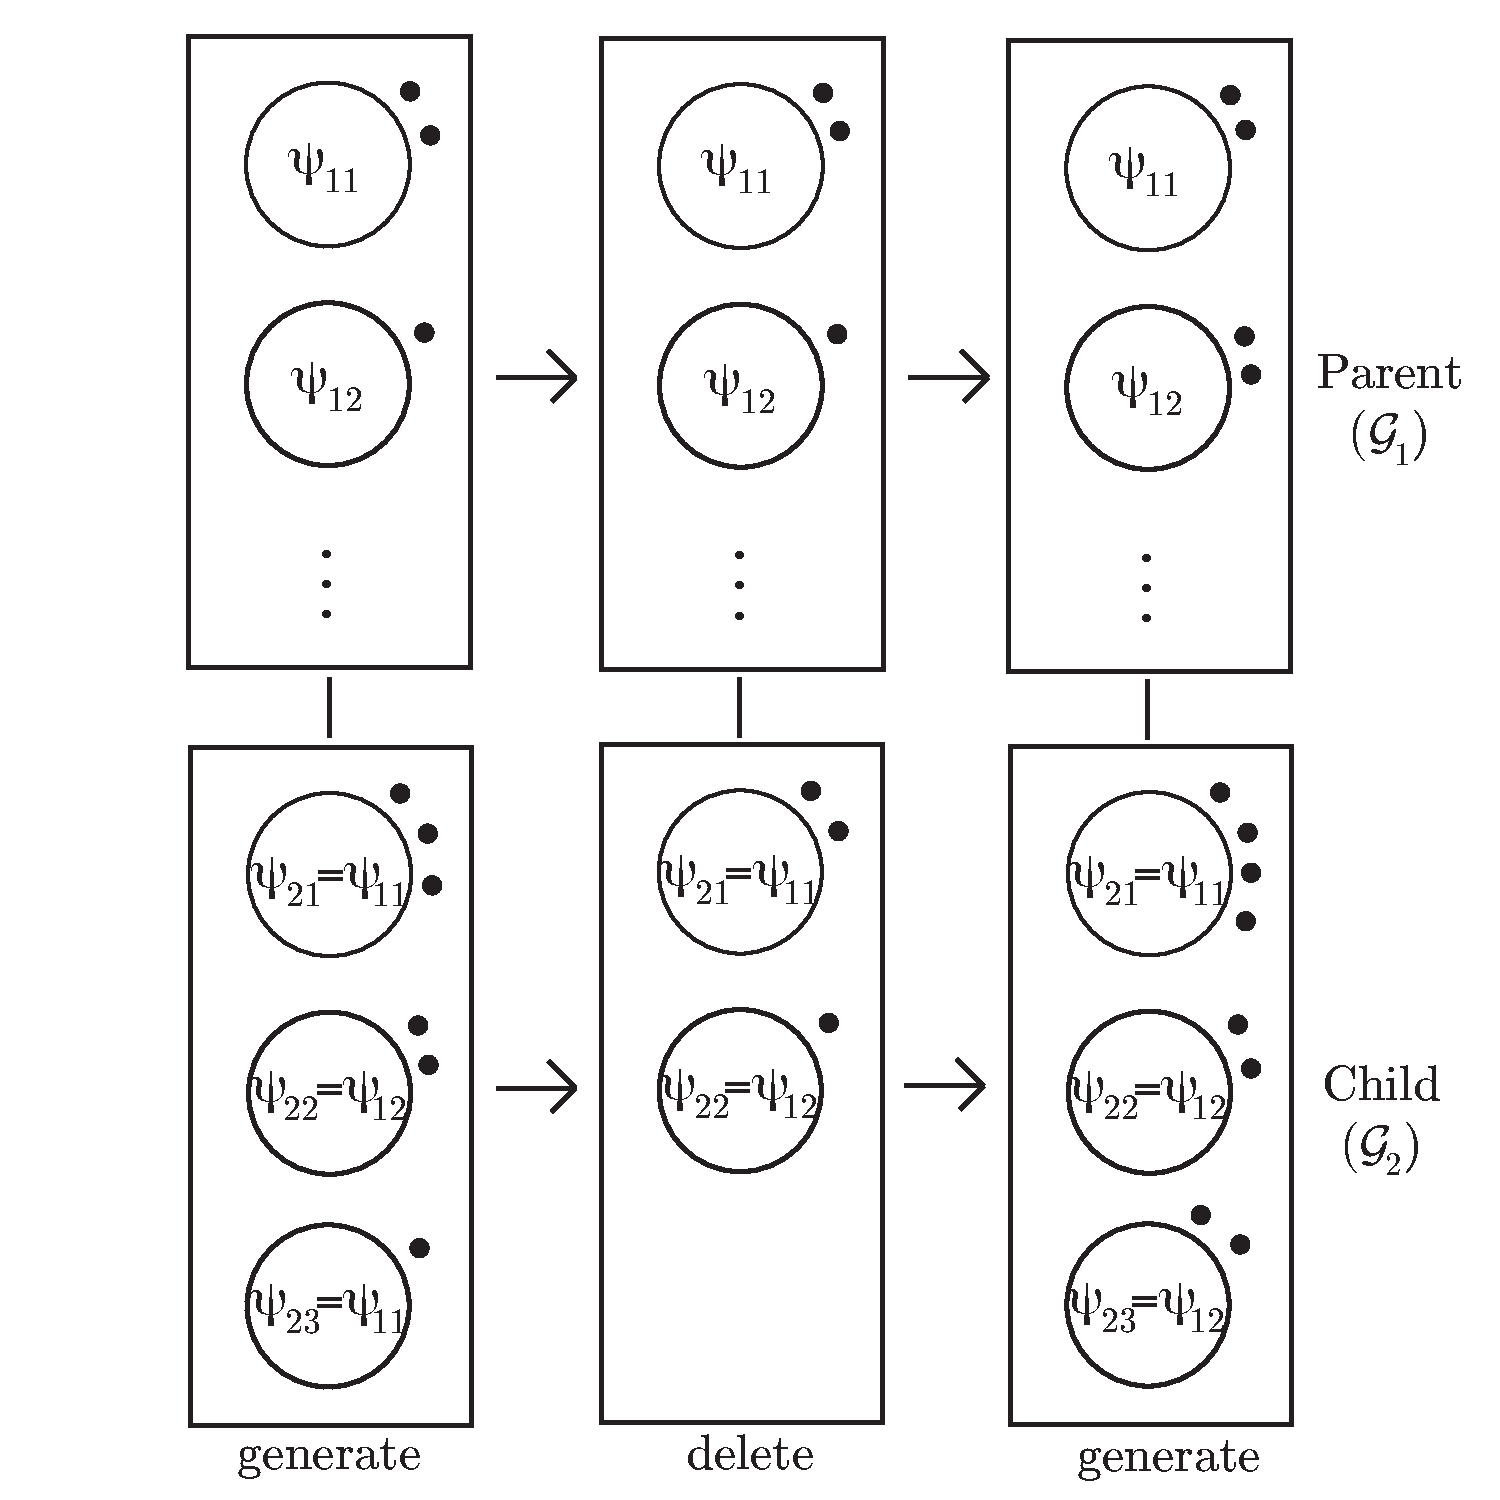
\includegraphics{figure2.pdf}} % [clip=true, viewport= 1in 1in 9in 9in]
		\caption{An example of the possible evolution of the restaurant states in a hierarchical setting}
		\label{figVHPY}
	\end{center} 
\end{figure} 

Figure~\ref{figVHPY} illustrates the potential evolution of the restaurants used during the CRF process modified to draw a sample from dependent distributions following a Pitman-Yor process distribution.  The middle column of restaurants show the restaurant customer configurations after a deletion step.  Note the configuration of the parent restaurant does not change even though one of the tables in the child restaurant has been removed.  The customer configuration in the third column shows a potential seating arrangement which could have generated the observed sample.  Here, a customer was added to the the parent restaurant in order to generate the parameter $\psi_{12}$  given to the third table in the child restaurant.

Simple extensions allowing for dependent distributions higher on the hierarchy are straightforward.  Given the model specification
%
\begin{eqnarray*}
\G_1^t | d_1, c_1, \G_0  &\sim& \PY(d_1,d_2,\G_0) \hspace{.5cm} t = 1\dots T\\
\G_2^t | d_2, c_2, \G_1^t &\sim& \PY(d_2, c_2, \G_1^t)  \hspace{.5cm} t = 1\dots T\\
\theta^t_i | \G_2^t &\sim& \G_2^t \hspace{.5cm} i = 1\dots N_t, 
\end{eqnarray*}
%
if we assume independence of the $\{ \G_2^t \}$ we can use the generalized restaurant procedure to generate samples. The assumption of independence indicates that at each time step the restaurant corresponding to $\G_2$ is emptied of all customers. Without the assumption of independence the extension is not straightforward. Creating a modified restaurant procedure to draw a sample from such a model would require a process to update the customer configuration in the restaurant corresponding to $\G_2$ to reflect changes made to the configuration of the restaurant corresponding to $\G_1$, while maintaining a level of dependence.  It is likely that such a process exists, but it is not necessary for this discussion.

\subsection{Time-varying model applied to SM}

The time-varying model will not only allow for a sequence of time-varying distributions, but can also serve to limit the complexity of the model representation. This framework provides a basis for algorithmic control of the complexity of hierarchical Pitman-Yor models like the SM.  As noted earlier, the number of instantiated restaurants in the SM is the fundamental limiting factor regarding memory usage, thus we will consider a single instantiated restaurant as a unit of memory when discussing the model. For the deletion scheme to limit the amount of memory used by the SM model, we must be able to limit the number of instantiated restaurants.

\begin{figure*}[t] 
	\begin{center}
		\scalebox{.4}{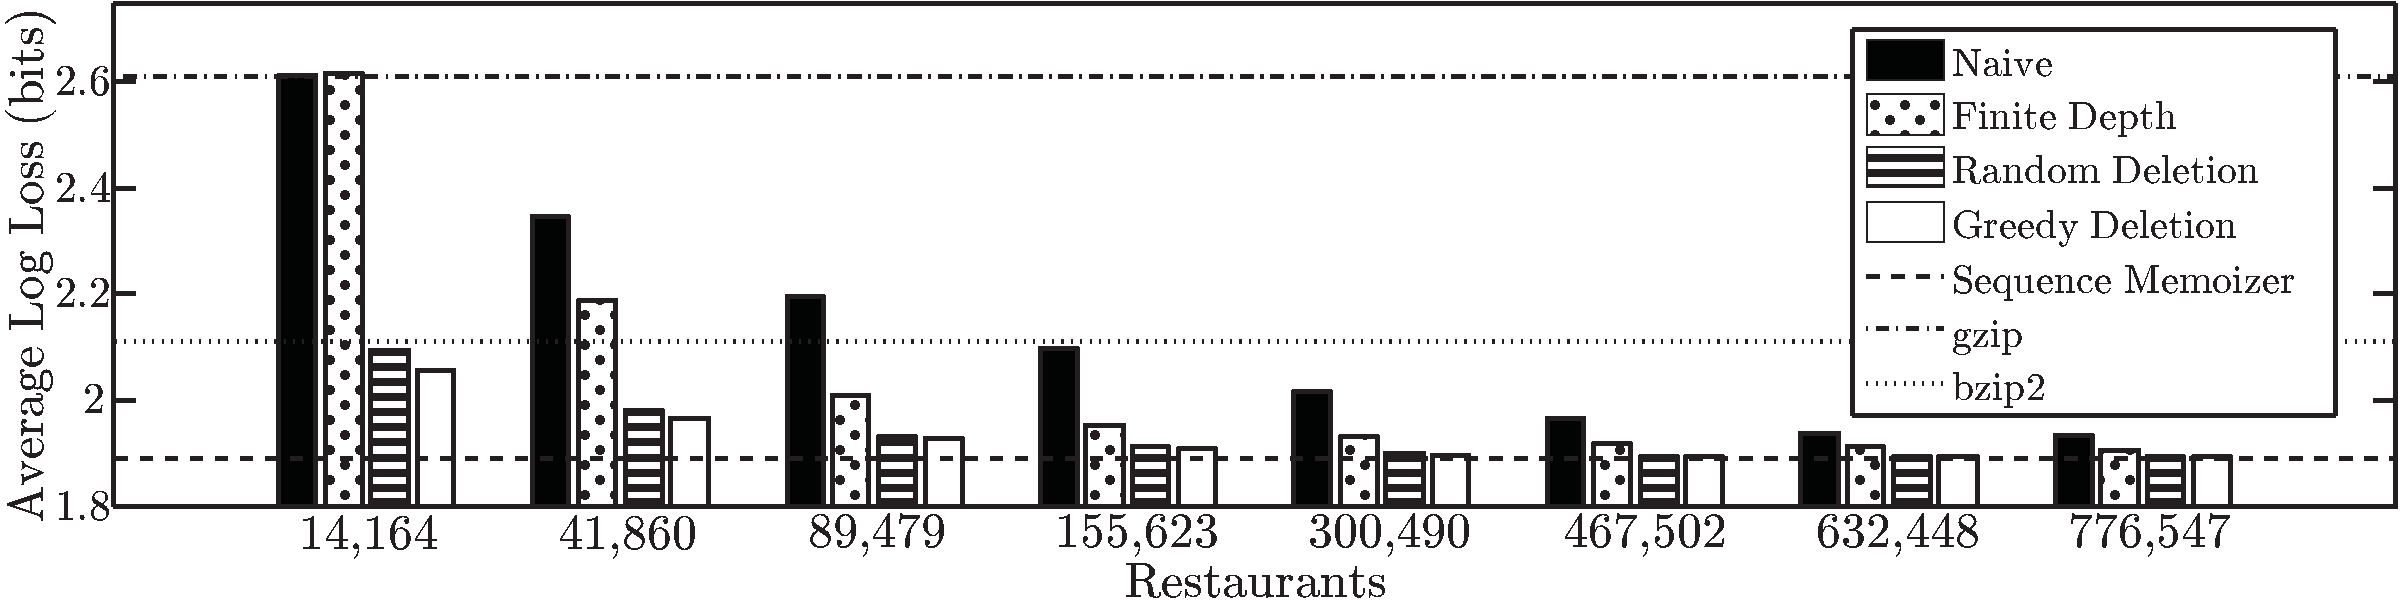
\includegraphics{results_calgary_corpus.pdf}} % [clip=true, viewport= 1in 1in 9in 9in]
		\caption{An example of the possible evolution of the restaurant states in a hierarchical setting}
		\label{figResultsCC}
	\end{center} 
\end{figure*} 

The theory presented above indicates that between time steps we can only delete customers in restaurants at the lowest level.  In the tree which represents the state of the SM, this corresponds to the leaf restaurants.  To achieve memory savings we will need to delete all of the customers at a given restaurant.  Restaurants without people need not be represented in the model state.  This deletion operation gives rise to implicit model assumptions. If, at time step $t$, we delete all the customers in a given leaf restaurant we implicitly assume the distribution over types given the particular context to be independent of the distribution at previous time steps.

It is often the case in the SM model that the parent restaurant for a leaf restaurant is not instantiated, thus to actually attain memory savings by deleting a leaf restaurant we must effectively delete all the restaurants in this particular path up until the nearest instantiated restaurant.  The implicit model assumption is that all of the distributions after time $t$ corresponding to those many deleted restaurants are conditionally independent of their previous states.

This is the basic framework for both bounded memory algorithms we present and is the main contribution of this paper.  The assumption that, for many contexts, the distribution changes over time seems appropriate for very long sequences. The assumption of independence required for us to justify our particular deletion process is primarily of practical motivation though we expect information lost to be minimal. 

Finally, we point out that the theory behind these deletion operations holds for general hierarchical Pitman-Yor processes and thus also for finite depth n-gram style models.  In Section~\ref{results} we show some results concerning this type of model as well.


\section{Inference}

Typically in these types of bayesian hierarchical models we would like to perform inference using MCMC sampling methods.  Here, the complexity of the model, and the desired use require online methods.  One natural approach is to use a particle filter given the sequential nature of the generative model.  The base SM model in our implementation is specified and estimated following the outline by [Gasthaus] using their 1PF approach.  That is, we use eleven unique, depth specific discount parameters where the eleventh discount is also the discount for larger depths.  The model is fit using a single particle particle filter and the discount parameters are optimized in a greedy sequential manner.  In the process of seating each observation we calculate the gradient of the predictive probability for the current observation with respect to the discount parameters and then step the discount parameters in the direction of the gradient.

To infer which restaurants to delete we have implemented two different methods.  Both methods are exploratory and are by no means exhaustive.  The first deletes leaf nodes completely at random.  Since we are using a single particle particle filter, this means that as soon as we delete the restaurants, we instantly free up memory.  At first, this deletion scheme seems a bit crude, but note that since we have only one particle, the available information for inferring which restaurants to delete is minimal.  

Our second method takes into account the log probability of the observed data given the current state of the model.  That is, given the current state of the model we can calculate the probability of generating exactly the sequence of data used to build the model.  By deleting different leaf restaurants the probability of the sequence, given the updated state of the model, changes.  We can rank the leaf restaurants in order by which deletions are least helpful regarding predicting the observed sequence and then delete those at the bottom of the ranking.  Since the current state of the model can be seen as a point estimate of the posterior distribution over the model space we consider this deletion scheme to be using, roughly, the useful idea of Bayes factors when deciding which restaurants to delete.

Given that the primary goal of this model is to limit the amount of memory required in the inference algorithm, we parameterized the implementation with an upper limit on the number of instantiated restaurants.  The implementation we used deletes 100 restaurants when the number of instantiated restaurants goes above the max number of restaurants allowed minus two in order to maintain a strict upper bound.  The number 100 was chosen arbitrarily and experimentation might be useful.

\subsection{Complexity}

A little consideration will show that both of the algorithms suggested for inference in this model require constant space, in the sense of the turing machine, and linear time.  The claim that the algorithms are linear in time stems from the fact that each observation must be seated, but now each seating operation is a constant time operation as the length of any path one must traverse in order to seat an observation is bounded by the total number of instantiated restaurants.  Furthermore, each deletion step requires, at worst, visiting every instantiated restaurant, which if done recursively is a constant time algorithm given that the number of instantiated restaurants is limited.  

The claim that the algorithm requires constant space requires a little more thought.  It is clear that we have limited the space required by restaurant objects, but what about the actual construction of the tree?  Currently our implementation labels each edge between nodes with two integers which index into the original sequence in order to describe that particular edge.  That is, if the parent restaurant corresponds to the distribution over bytes following $oc$,  and the child restaurant corresponds to the distribution over bytes following $acdoc$, the connecting path may be described by the integer array $[17,20]$ if in the sequence being seated, the entries 18-20 are $acd$.  This type of algorithm requires only constant space for each edge, though it works best if the entire sequence is held in memory.  That being said, considering the sequence being seated to be a semi-infinite tape as in the turing machine stipulation, reversals of the tape are allowable.  Thus, the entire sequence need not be held in memory, it is only necessary that we can reverse the tape to access previous entries in the sequence if we need them.

As a practical side note, an alternative approach to implementation could store the full connecting context on the edge between nodes.  In the above example this would correspond to labeling the edge with the byte array $[acd]$.  While this does not theoretically require constant space, typically when implementing the algorithm on real data only a short section at the end the array is used.  Caching a fixed length section of the each array on the appropriate edge could drastically reduce the number of times the algorithm requires the tape to reverse.  As an example, if one was fitting the entire model on each document of the calgary corpus separately, as we do in the results section, and were willing to cache arrays of length 6,000, a tape reversal would never be required.  This number could only decrease using either of the deletion schemes suggested.  Finally, if we use a fixed depth model, caching the contexts on the edges requires only constant memory when enforcing an upper bound on the number of restaurants.


\section{Experiments and results}
\label{results}

The data we used for the first experiment was the Calgary Corpus \cite{calgary corp}.  The Calgary Corpus is made up of 14 separate documents meant to simulate the task of compression in a general setting. Documents were modeled separately as a sequence of bytes.  Results are reported as corpus wide average log-loss in bits.  In the compression setting this corresponds directly to compression ratio.

%\label{figResultsCC}

To baseline our model we ran two other constant space sequence models and two standard compressors.  The first was an adaptation of the SM model to finite depths.  By bounding the depth of the SM we create a finite depth HPYP model with concentration parameters zero.  Inference was performed using the single particle particle filter. The second was a naive constant space modeling technique using the SM to model.  When the number of instantiated restaurants in the model reached the threshold the remainder of the sequence was modeled with a separate SM model.  We also compressed each file using gzip and bzip2 \cite{gzip} \cite{bzip2}.  Default parameters were used for the commercial compressors.

The first step of the experiment was to model each document in the corpus with finite depth SM models of depths 2 through 9.  For each document and model we recorded the number of instantiated restaurants in the final state of the model.  The document requiring the largest number of instantiated restaurants provides an implicit bound on the space required to model the corpus as a whole. The implicit bound specific to each depth was then used as a threshold in the SM model paired with the two deletion schemes proposed in Section~\ref{inference}. This method of comparison was used because the standard finite depth models do not permit a space upper bound specification a priori.

Each of the four sequence models were fit ten times to understand the variance of the inference procedure.  Our results show the standard deviation of the average log loss to be less than $0.002$ for all of the methods.  All differences detectable in the graph are significant at the $\alpha = 0.01$ level. We note that the SM model paired with either deletion scheme consistently out performs the finite depth model.  Furthermore, the greedy deletion scheme shows improvement over the random deletion scheme, especially for low thresholds.  The SM model paired with either deletion scheme outperformed the commercial compressors at every threshold tested.

\section{Discussion}
\label{discussion}

In the course of this paper we developed a generative model for a dependent HPYP. This model is amenable to sequential Monte Carlo estimation.  We know that other ways to generate dependent HPYP's will emerge, and hope that others too will be amenable to efficient incremental inference techniques.  We explained how dependency in our specific dependent HPYP formulation arises from deleting whole restaurants in a Chinese restaurant franchise representation.  We show that this restaurant deletion scheme can be either be deterministic or probabilistic.  In contrast to others who have used deletion in Chinese restaurant representations to induce dependence between processes we suggested using a deterministic deletion policy to control the memory complexity of inference.  The utility of our predictive model seems promising, particularly when considering how it might be used in a probabilistic lossless compressor.  This is because the performance of the constant memory models is nearly indistinguishable from that of state of the the art sequence models and significantly better than that of existing commercial compressors.

The techniques highlighted in this paper point to interesting avenues for future research.  In essence the restaurant forgetting scheme amounts to a greedy stochastic approach to graphical model structure learning.  As data continually arrives, only those graphical model nodes corresponding to contexts that are both meaningful and continually reappear will remain in the graphical model after many deletion operations.   While the deletion scheme utilized in this work is highlighted in the context of a single family of models corresponding to a single graphical model architecture, it may be possible to use deletion operations in models of more general architecture.

\bibliography{../../uber.bib}
\bibliographystyle{icml2010}

\end{document} 
